%%%%%%%%%%%%%%%%%%%%%%%%%%%%%%%%%%%%%%%%%
% Beamer Presentation
% LaTeX Template
% Version 1.0 (10/11/12)
%
% This template has been downloaded from:
% http://www.LaTeXTemplates.com
%
% License:
% CC BY-NC-SA 3.0 (http://creativecommons.org/licenses/by-nc-sa/3.0/)
%
%%%%%%%%%%%%%%%%%%%%%%%%%%%%%%%%%%%%%%%%%

%----------------------------------------------------------------------------------------
%	PACKAGES AND THEMES
%----------------------------------------------------------------------------------------

\documentclass[10pt]{beamer}

\mode<presentation> {

% The Beamer class comes with a number of default slide themes
% which change the colors and layouts of slides. Below this is a list
% of all the themes, uncomment each in turn to see what they look like.

%\usetheme{default}
%\usetheme{AnnArbor}
%\usetheme{Antibes}
%\usetheme{Bergen}
%\usetheme{Berkeley}
%\usetheme{Berlin}
%\usetheme{Boadilla}
%\usetheme{CambridgeUS}
%\usetheme{Copenhagen}
%\usetheme{Darmstadt}
%\usetheme{Dresden}
%\usetheme{Frankfurt}
%\usetheme{Goettingen}
%\usetheme{Hannover}
%\usetheme{Ilmenau}
%\usetheme{JuanLesPins}
%\usetheme{Luebeck}
\usetheme{Madrid}
%\usetheme{Malmoe}
%\usetheme{Marburg}
%\usetheme{Montpellier}
%\usetheme{PaloAlto}
%\usetheme{Pittsburgh}
%\usetheme{Rochester}
%\usetheme{Singapore}
%\usetheme{Szeged}
%\usetheme{Warsaw}

% As well as themes, the Beamer class has a number of color themes
% for any slide theme. Uncomment each of these in turn to see how it
% changes the colors of your current slide theme.

%\usecolortheme{albatross}
%\usecolortheme{beaver}
%\usecolortheme{beetle}
%\usecolortheme{crane}
%\usecolortheme{dolphin}
%\usecolortheme{dove}
%\usecolortheme{fly}
%\usecolortheme{lily}
%\usecolortheme{orchid}
%\usecolortheme{rose}
%\usecolortheme{seagull}
%\usecolortheme{seahorse}
%\usecolortheme{whale}
%\usecolortheme{wolverine}

%\setbeamertemplate{footline} % To remove the footer line in all slides uncomment this line
%\setbeamertemplate{footline}[page number] % To replace the footer line in all slides with a simple slide count uncomment this line

\setbeamertemplate{navigation symbols}{} % To remove the navigation symbols from the bottom of all slides uncomment this line
}

\usepackage{graphicx} % Allows including images
\usepackage{booktabs} % Allows the use of \toprule, \midrule and \bottomrule in tables
\usepackage{hyperref}
\usepackage{tikz}
\usepackage{algpseudocode}
\usepackage{algorithm}
\usepackage{multicol}
\setbeamerfont{frametitle}{size=\large}
\setbeamerfont{framesubtitle}{size=\small}
\setbeamertemplate{caption}[numbered]

%----------------------------------------------------------------------------------------
%	TITLE PAGE
%----------------------------------------------------------------------------------------

\title[Cooperative Explorer]{COEX-1} % The short title appears at the bottom of every slide, the full title is only on the title page
\subtitle{Cooperative Explorer}
\author[Aurélien Werenne]{Aurélien Werenne \\ {\small Advisor: Prof. B. Boigelot}} 
\institute[ULiège] 
{
University of Liège \\ 
\medskip
Link to code: \href{https://github.com/Werenne/multi-agent-mapping}{\textcolor{blue}{Github}}

}
\date{\today} 

\begin{document}

\begin{frame}
\titlepage 
\end{frame}

\begin{frame}
\frametitle{Overview} 
\tableofcontents 
\end{frame}

%----------------------------------------------------------------------------------------
%	PRESENTATION SLIDES
%----------------------------------------------------------------------------------------

%------------------------------------------------
\section{General} 
%------------------------------------------------

\begin{frame}
\frametitle{Overview}
\tableofcontents[currentsection,subsectionstyle=shaded]
\end{frame}

%------------------------------------------------
\begin{frame}
\frametitle{General}
\framesubtitle{Objective}
The goal of the robot, named COEX-1, is to perform a mapping of an unknown environment. The robot cooperates in a centralized multi-agent setting. \\~\\
The main features of the robot are:
\begin{itemize}
\item Following a black line
\item Computing the travelled distance
\item Detecting, classifying and handling intersections
\item Avoiding obstacles
\item Communication with the central unit 
\end{itemize}
\end{frame}

%------------------------------------------------
\begin{frame}
\frametitle{General}
\framesubtitle{Material}
Non-exhaustive list of used components:
\begin{itemize}
\item Microcontroller (Arduino Nano) 
\item Reflectance sensor array (Pololu QTR-MD-06A)
\item Digital distance sensor (Sharp GP2Y)
\item Magnetic encoders 
\item DC Motor (Pololu 150:1 micro metal gearmotor MP)
\item Motor driver (L298N dual H-bridge) 
\item Battery (NiMH 7.2V) 
\item Bluetooth module (HC-05) 
\end{itemize}
\end{frame}

%------------------------------------------------

\begin{frame}
\frametitle{General}
\framesubtitle{Structure (1/3)}
\begin{figure}[hbtp]
\centering
\begin{tikzpicture}
	\node [anchor=west] (bluetooth) at (-1.6,5) {\small Bluetooth};
	\node [anchor=west] (nano) at (-1.6,3) {\small Nano};
	\node [anchor=west] (sharp) at (-1.6,1) {\small Sharp};
	\node[anchor=south west,inner sep=0] (image) at (0,0) {\includegraphics[scale=0.05]{figures/img_front.JPG}};
	\begin{scope}[x={(image.south east)},y={(image.north west)}]
		%\draw[help lines,xstep=.1,ystep=.1] (0,0) grid (1,1);
		\draw[yellow,ultra thick,rounded corners] (0.62,0.25) rectangle (0.72,0.40);
		\draw[yellow,ultra thick,rounded corners] (0.35,0.60) rectangle (0.45,0.83);
		\draw[yellow,ultra thick,rounded corners, rotate around={48:(0.55,0.50)}] (0.55,0.50) rectangle (0.65,0.70);
		\draw [-latex, ultra thick, yellow] (bluetooth) to[out=0, in=-120] (0.35,0.6);
		\draw [-latex, ultra thick, yellow] (nano) to[out=0, in=-120] (0.5,0.55);
		\draw [-latex, ultra thick, yellow] (sharp) to[out=0, in=-160] (0.62,0.32);
	\end{scope}
\end{tikzpicture}
\caption{Front view of COEX-1}
\end{figure}
%
\end{frame}

%------------------------------------------------

\begin{frame}
\frametitle{General}
\framesubtitle{Structure (2/3)}
\begin{figure}[hbtp]
\centering
\begin{tikzpicture}
	\node [anchor=west] (battery) at (-1.6,5) {\small Battery};
	\node [anchor=west] (shield) at (-1.6,3) {\small Shield};
	\node[anchor=south west,inner sep=0] (image) at (0,0) {\includegraphics[scale=0.05]{figures/img_side.JPG}};
	\begin{scope}[x={(image.south east)},y={(image.north west)}]
		%\draw[help lines,xstep=.1,ystep=.1] (0,0) grid (1,1);
		\draw[yellow,ultra thick,rounded corners] (0.65,0.35) rectangle (0.75,0.62);
		\draw[yellow,ultra thick,rounded corners] (0.38,0.23) rectangle (0.55,0.35);
		\draw [-latex, ultra thick, yellow] (battery) to[out=0, in=120] (0.65,0.62);
		\draw [-latex, ultra thick, yellow] (shield) to[out=0, in=-120] (0.38,0.23);
	\end{scope}
\end{tikzpicture}
\caption{Side view of COEX-1}
\label{fig:fig-img-side}
\end{figure}
\end{frame}

%------------------------------------------------

\begin{frame}
\frametitle{General}
\framesubtitle{Structure (3/3)}
\begin{figure}[hbtp]
\centering
\begin{tikzpicture}
	\node [anchor=west] (array) at (-2.6,5) {\small Reflectance array};
	\node [anchor=west] (motors) at (-1.6,3) {\small Motors};
	\node[anchor=south west,inner sep=0] (image) at (0,0) {\includegraphics[scale=0.048]{figures/img_bottom.JPG}};
	\begin{scope}[x={(image.south east)},y={(image.north west)}]
		%\draw[help lines,xstep=.1,ystep=.1] (0,0) grid (1,1);
		\draw[yellow,ultra thick,rounded corners] (0.47,0.5) rectangle (0.68,0.65);
		\draw[yellow,ultra thick,rounded corners] (0.38,0.11) rectangle (0.75,0.25);
		\draw [-latex, ultra thick, yellow] (array) to[out=0, in=120] (0.47,0.65);
		\draw [-latex, ultra thick, yellow] (motors) to[out=0, in=150] (0.55,0.25);
	\end{scope}
\end{tikzpicture}
\caption{Bottom view of COEX-1}
\label{fig:fig-img-bottom}
\end{figure}
\end{frame}

%------------------------------------------------

\begin{frame}
\frametitle{General}
\framesubtitle{Nomenclature}
Let us define some terminology,
\begin{itemize}
\item \textit{Error line}: the deviation (in cm) of the detected black line from the center of the sensor array ($err_{line} \in [-2;2]$).
\item \textit{Target speed}: the speed the robot wants to achieve.
\item \textit{Progress speed}: an intermediate value of speed whose value is in between the previous and the current target speed. Serves as a proxy to smoothly control acceleration.
\item \textit{Measured speed}: the speed measured by the encoder, i.e. the actual speed of COEX-1.
\end{itemize}
\end{frame}

%------------------------------------------------
\section{Components} 
%------------------------------------------------

\begin{frame}
\frametitle{Overview}
\tableofcontents[currentsection,subsectionstyle=shaded]
\end{frame}

%------------------------------------------------
\begin{frame}
\frametitle{Components}
\framesubtitle{Sharp sensor}
Adding a bypass capacitor was necessary to make the Sharp sensor work. On Fig.\ref{fig:sharp-flow} the detection of obstacles is read perfectly. The threshold is set at 2 Volt instead of the mean (3 Volt) in order to avoid False Negatives.
\vspace*{-2mm}
\begin{figure}[hbtp]
\centering
\includegraphics[scale=0.45]{figures/sharp-flow.png}
\vspace*{-2mm}
\caption{Sharp sensor output, $f=20Hz$. Test performed with back and forth movement of obstacle, going in and out of reach of the sensor.}
\label{fig:sharp-flow}
\end{figure}
\end{frame}


%------------------------------------------------

\begin{frame}
\frametitle{Components}
\framesubtitle{Reflectance sensor array (line sensor)}
Experimentally, I found it is best to average four readings of the sensor to reduce noise. By doing so, we can observe the sensor's output varying smoothly. The sensor is particularly sensitive to ambient light interferences. As a solution a shield was constructed around the sensor (Fig.\ref{fig:fig-img-bottom}).
\vspace*{-2mm}
\begin{figure}[hbtp]
\centering
\includegraphics[scale=0.42]{figures/qtr-flow.png}
\vspace*{-4mm}
\caption{QTR sensor output, $f=100Hz$. Test performed by moving the black line back and forth between left and right side of the sensor.}
\label{fig:flow-qtr}
\end{figure}
\end{frame}

%------------------------------------------------

\begin{frame}
\frametitle{Components}
\framesubtitle{Bluetooth module (1/5)}
To evaluate the robustness of the communication protocol, a simple test is performed which I call the \textit{sinus test}. The principle is to send a message at time $t$ with content $f(t)$ to the robot, and receive its response at time $t'$ with content $f(t)$ unchanged. The function $f(t) = A\sin(2\frac{\pi}{T}t)+b$, enables us to easily deduce delay. \\~\\
On Figs \ref{fig:sinus-i-5}, \ref{fig:sinus-i-25}, \ref{fig:sinus-i-40} we plot $(t,f(t))$ and on Figs \ref{fig:sinus-o-5}, \ref{fig:sinus-o-25}, \ref{fig:sinus-o-40} we plot $(t',f(t))$. We conclude that 5Hz works well and is enough for our use case.
\end{frame}

%------------------------------------------------

\begin{frame}
\frametitle{Components}
\framesubtitle{Bluetooth module (2/5)}
\begin{multicols}{2}
\begin{figure}
\centering
\includegraphics[scale=0.4]{figures/sending-5hz.png}
\caption{Sinus test at 5Hz, input signal}
\label{fig:sinus-i-5}
\end{figure}
\columnbreak
\begin{figure}
\centering
\includegraphics[scale=0.4]{figures/reception-5hz.png}
\caption{Sinus test at 5Hz, output signal}
\label{fig:sinus-o-5}
\end{figure}
\end{multicols}
\end{frame}

%------------------------------------------------

\begin{frame}
\frametitle{Components}
\framesubtitle{Bluetooth module (3/5)}
Some loss is observed at 25Hz.
\begin{multicols}{2}
\begin{figure}
\centering
\includegraphics[scale=0.4]{figures/sending-25hz.png}
\caption{Sinus test at 25Hz, input signal}
\label{fig:sinus-i-25}
\end{figure}
\columnbreak
\begin{figure}
\centering
\includegraphics[scale=0.4]{figures/reception-25hz.png}
\caption{Sinus test at 25Hz, output signal}
\label{fig:sinus-o-25}
\end{figure}
\end{multicols}
\end{frame}

%------------------------------------------------

\begin{frame}
\frametitle{Components}
\framesubtitle{Bluetooth module (4/5)}
At 40Hz, the protocol completely breaks down.
\begin{multicols}{2}
\begin{figure}
\centering
\includegraphics[scale=0.4]{figures/sending-40hz.png}
\caption{Sinus test at 40Hz, input signal}
\label{fig:sinus-i-40}
\end{figure}
\columnbreak
\begin{figure}
\centering
\includegraphics[scale=0.4]{figures/reception-40hz.png}
\caption{Sinus test at 40Hz, output signal}
\label{fig:sinus-o-40}
\end{figure}
\end{multicols}
\end{frame}
%------------------------------------------------

\begin{frame}
\frametitle{Components}
\framesubtitle{Bluetooth module (5/5)}
A voltage divider was added to the circuit because of the difference between the logic level voltage of the Arduino ($0-5$ Volt) and the bleutooth module ($0-3.3$ Volt). 
\begin{columns}[c]

\column{.35\textwidth}
\begin{align*} 
V_{arduino} &=  \frac{R_2}{R_1+R_2}V_{bleutooth} \\[0.4cm]
 &=  \frac{2.2}{3.2}V_{bleutooth}
\end{align*}

\column{.65\textwidth}
\begin{figure}[hbtp]
\centering
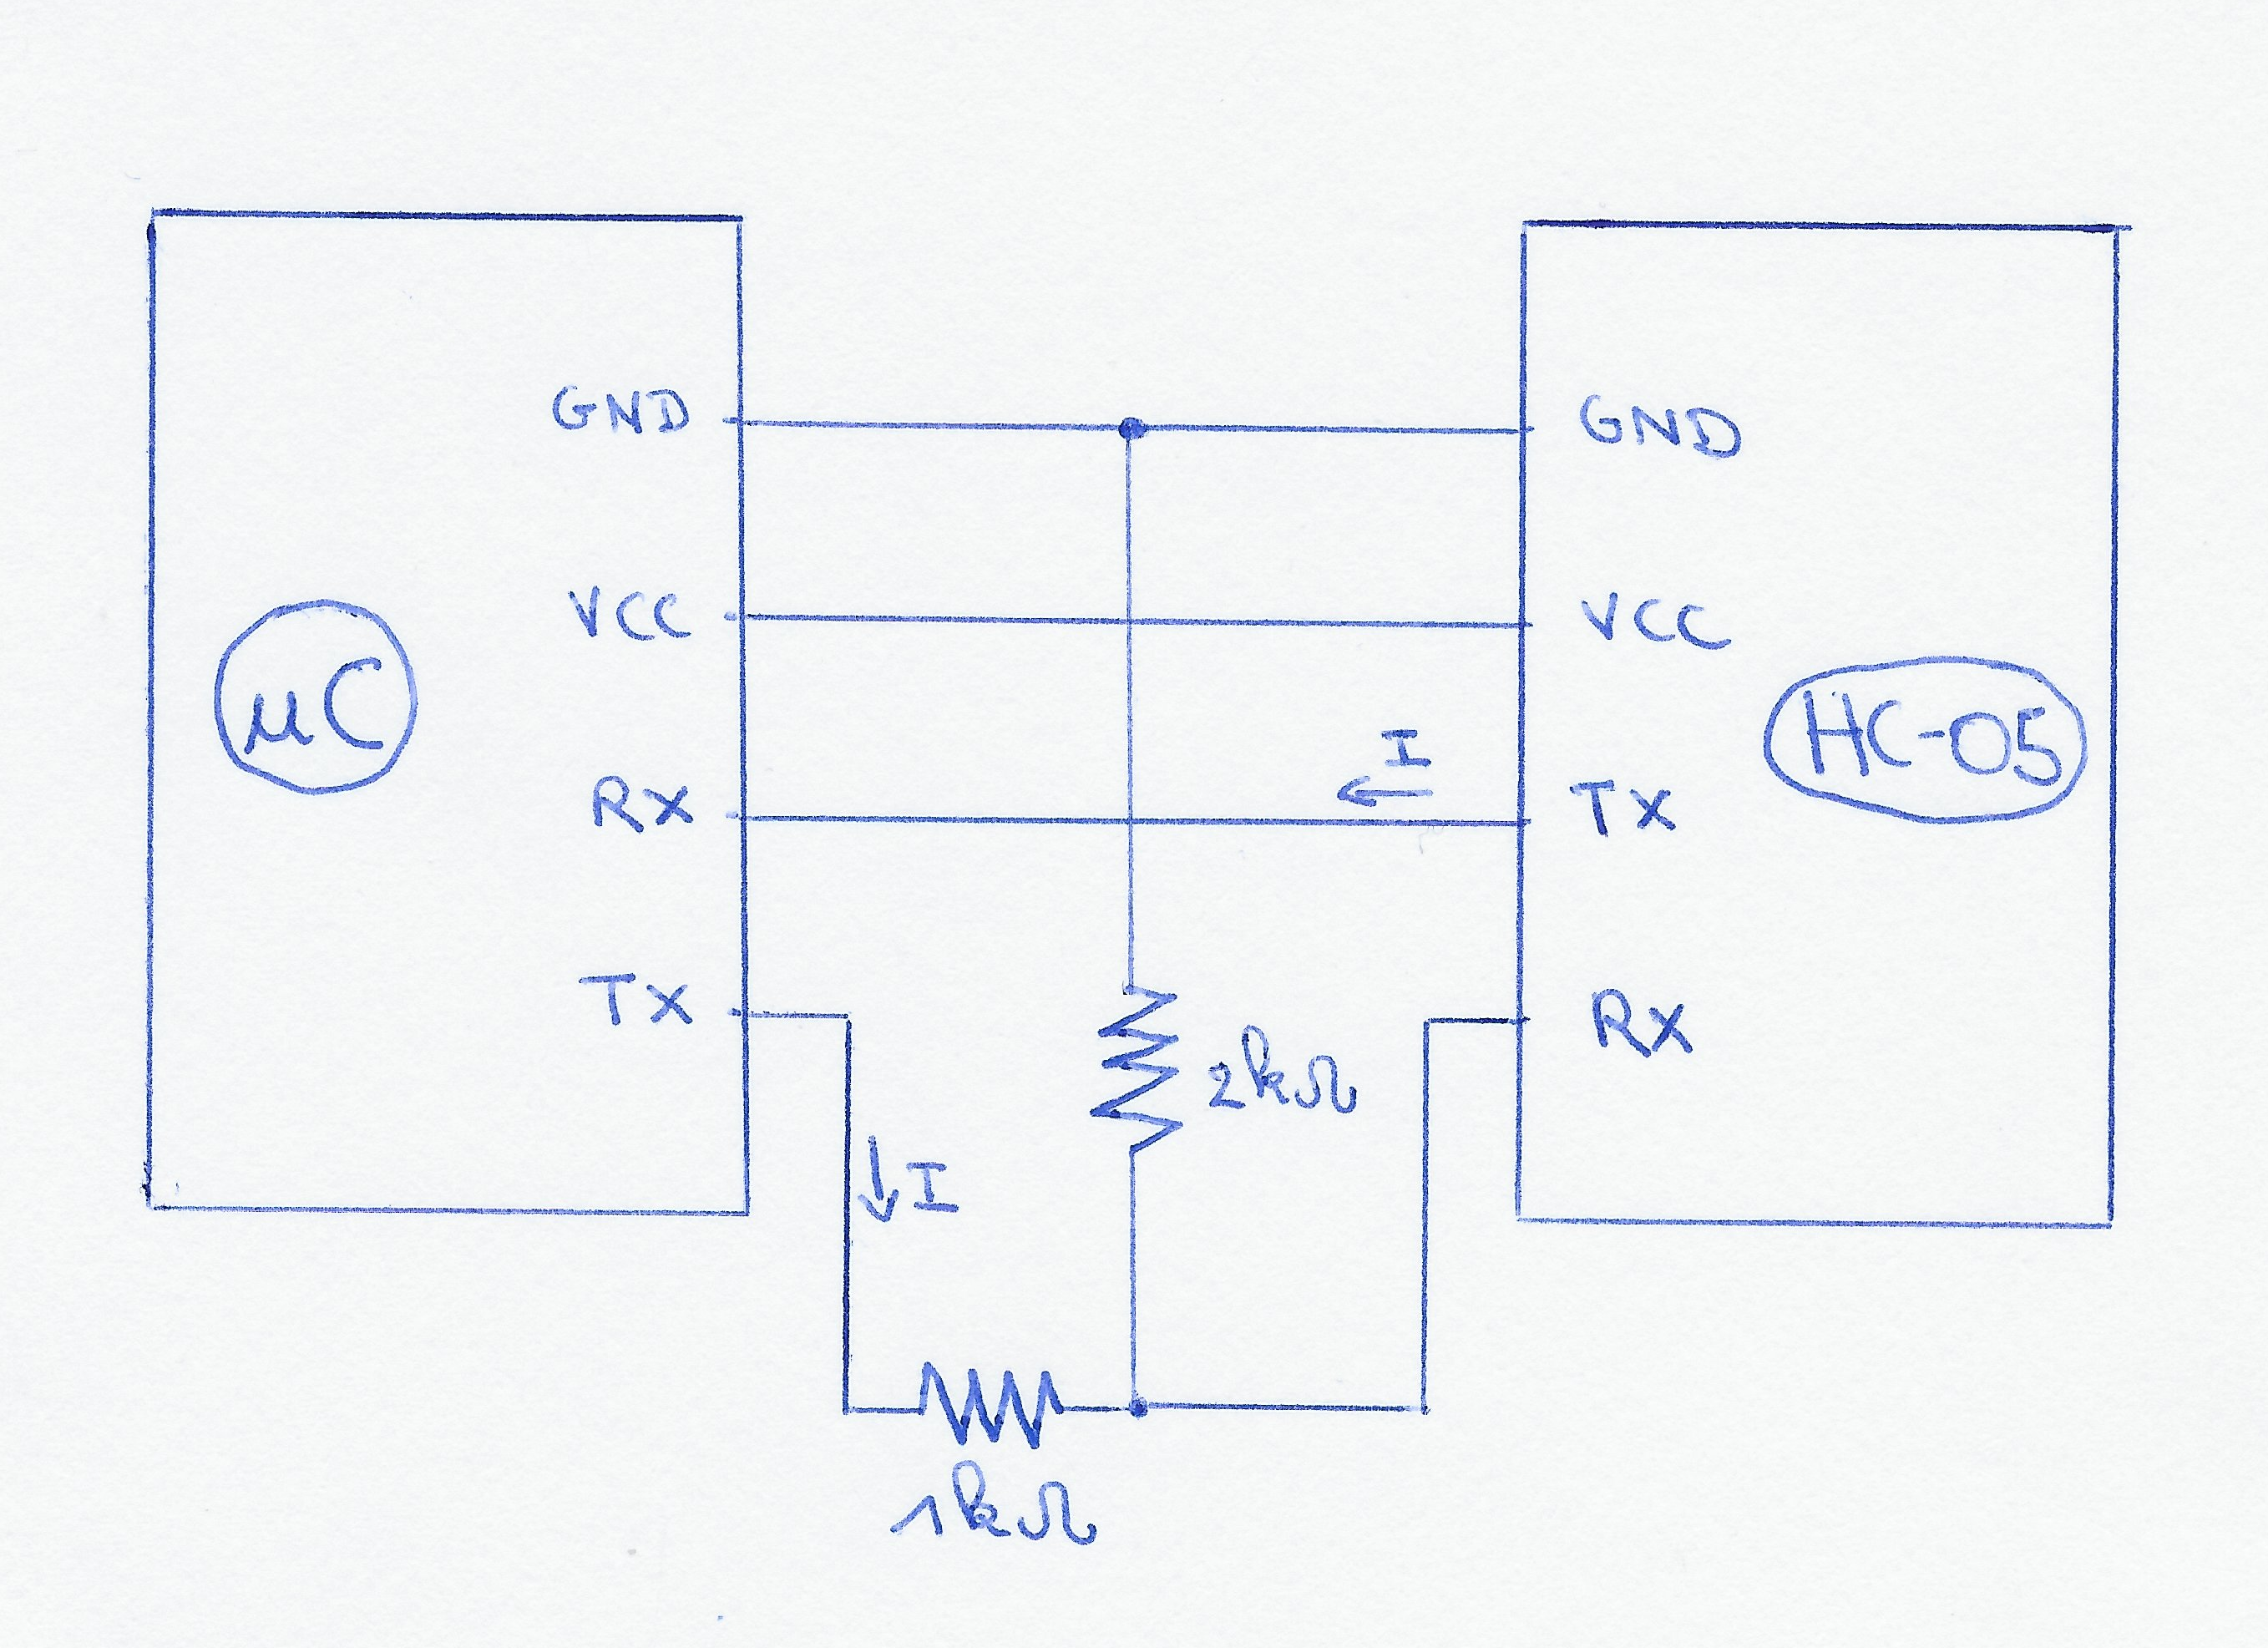
\includegraphics[scale=0.07]{figures/diag-voltage-divider}
\caption{Voltage divider}
\end{figure}

\end{columns}
\end{frame}

%------------------------------------------------

\begin{frame}
\frametitle{Components}
\framesubtitle{Quadrature encoders (1/2)}
Making use of the Hall effect, the encoders counts the number of revolutions of each motor shaft, noted $n_L$ and $n_R$. The angular velocity of the wheel is computed as follows:
$$ 
w_L = 2\pi f_L
\qquad\text{with}\qquad	
f_L = \frac{n_L}{N\, G_b \, \Delta{t} }
$$
with $N$ the number of counts per revolution on one channel\footnote{Having only 2 interrupt pins available on the Arduino Nano, only one channel of each encoder was used.}, and $G_b$ the gearbox ratio. The robot can be modelled as a differential steering wheel such that,
$$ 
v = \frac{v_L + v_R}{2} = \frac{R(w_L + w_R)}{2}
$$
\end{frame}

%------------------------------------------------

\begin{frame}
\frametitle{Components}
\framesubtitle{Motors}
The PWM is the signal send to the motors to control the speed. This relationship is visualized in the plot below. Small differences appear between the motors. We also note the variation with the charge of the battery. These imperfections force us to design a control-feedback system. 
\vspace*{-2mm}
\begin{figure}[hbtp]
\centering
\includegraphics[scale=0.45]{figures/motors_merged.png}
\vspace*{-2mm}
\caption{Relationship between PWM (input) and measured speed (output)}
\label{fig:pwm-speed}
\end{figure}
\end{frame}


%------------------------------------------------
\section{Control} 
%------------------------------------------------

\begin{frame}
\frametitle{Overview}
\tableofcontents[currentsection,subsectionstyle=shaded]
\end{frame}

%------------------------------------------------
\begin{frame}
\frametitle{Control}
\framesubtitle{General framework (1/2)}
A self-regulated system is acheived by using several PID controllers. The output of a PID controller can be expressed as
$$ 
o_n (e_0...e_n) \leftarrow K_p e_n + K_d\frac{e_n - e_{n-1}}{\Delta t_{n-1:n}} + \overbrace{K_e\sum_{i=0}^{n}{e_i \Delta t_{n-1:n}}}^{I_{out}^{(n)}}
$$
with anti-windup,
$$
I_{out}^{(n)} = \left\{
    \begin{array}{ll}
        max & \mbox{if } I_{out}^{(n)} > max \\
        min & \mbox{if } I_{out}^{(n)} < min \\
        I_{out}^{(n)} & \mbox{otherwise.}
    \end{array}
\right.
$$
\end{frame}

%------------------------------------------------

\begin{frame}
\frametitle{Control}
\framesubtitle{General framework (2/2)}
The three main controllers are used to control speed, direction and turning (discussed respectively on slides \ref{frame:control-speed}, \ref{frame:control-direction} and \ref{frame:control-turn}) \\~\\
The pwm value is computed from the three controllers outputs as
$$ 
\left\{
    \begin{array}{ll}
		\alpha = o(e_{direction}) \\[0.3cm]
		\beta = o(e_{speed}) \\[0.3cm]
		\gamma = o(e_{align})
	\end{array}
\right.
\Rightarrow
\left\{
    \begin{array}{ll}
		{pwm}_L =  (\beta -\gamma) + \alpha \\
		{pwm}_R = (\beta - \gamma) - \alpha
	\end{array}
\right.
$$
\end{frame}

%------------------------------------------------

\begin{frame}[label={frame:control-speed}]
\frametitle{Control}
\framesubtitle{Speed control (1/5)}
During speed control the systrem objective is to minimize $e_{speed}$, the difference between progress and measured speed. For a unifrom acceleration (shown in Fig.\ref{fig:uniform-acc}) the update rule for the progress speed is Eq.\ref{eq:update-uniform}
\begin{columns}[c]

\column{.55\textwidth}
\begin{figure}[hbtp]
\centering
\includegraphics[scale=0.07]{figures/uniform-acc}
\caption{Profile function of a uniform acceleration.}
\label{fig:uniform-acc}
\end{figure}

\column{.40\textwidth}
\hspace*{-10mm}
\begin{equation}\label{eq:update-uniform}
\begin{aligned}
&v_{n+1} \leftarrow v_n + A \, \Delta t_{n:n+1}\\
&\text{with}\,\ A = \frac{v_{target}}{T}
\end{aligned}
\end{equation}

\end{columns}
\end{frame}

%------------------------------------------------

\begin{frame}
\frametitle{Control}
\framesubtitle{Speed control(2/5)}
For a smoother transition\footnote{Design purely based on instinct, effectiveness of method needs to be confirmed by experiments.}, the robot accelerates following the profile as in Fig.\ref{fig:smooth-acc}. However, we want the robot to achieve the target speed in the same amount of time $T$. This constraint is developed in Eq.\ref{eq:constraint-smooth}.
\begin{columns}[c]

\column{.45\textwidth}
\begin{equation}\label{eq:constraint-smooth}
\begin{aligned}
&\Leftrightarrow \int_{0}^{T}a(t) =  \int_{0}^{T}a'(t) \\
&\Leftrightarrow A\,T = \underbrace{d\,B}_{triangles} + \underbrace{(T - 2d)B}_{rectangle}
\end{aligned}
\end{equation}

\column{.50\textwidth}
\begin{figure}[hbtp]
\centering
\includegraphics[scale=0.07]{figures/smooth-acc}
\caption{Profile function of a "smooth" acceleration}
\label{fig:smooth-acc}
\end{figure}
\end{columns}
\end{frame}

%------------------------------------------------

\begin{frame}
\frametitle{Control}
\framesubtitle{Speed control (3/5)}
By substituting the parameter $\psi = \frac{d}{T}$ in equation \ref{eq:constraint-smooth}, we obtain
$$
\boxed{B = \frac{A}{1-\psi}} 
$$
The update rule for the progress speed becomes
$$
v_{n+1} \leftarrow v_n + \int_{n}^{n+1}a'(t) = v_n + \int_{0}^{n+1}a'(t) - \int_{0}^{n}a'(t)
$$
Note that with the right hand side of the above expression, we can make use of precomputed values of the geometric surfaces.
\end{frame}

%------------------------------------------------

\begin{frame}
\frametitle{Control}
\framesubtitle{Speed control (4/5)}
The system achieves good results. Still, future tuning is necessary.
\begin{figure}[hbtp]
\centering
\includegraphics[scale=0.45]{figures/pid_speed_normal.png}
\caption{Evolution of measured with changing progress speed.}
\label{fig:all-cycles}
\end{figure}
\end{frame}

%------------------------------------------------

\begin{frame}
\frametitle{Control}
\framesubtitle{Speed control (5/5)}
To capture the general tendency, an average over all the cycles of Fig.\ref{fig:all-cycles} on the previous slide is done. 
\begin{figure}[hbtp]
\centering
\includegraphics[scale=0.45]{figures/pid_speed_shaded.png}
\caption{Mean measured speed with error band ($\pm 2$ standard deviation).}
\label{fig:average-pid}
\end{figure}
\end{frame}

%------------------------------------------------

\begin{frame}[label={frame:control-direction}]
\frametitle{Control}
\framesubtitle{Direction control (1/4)}
We define three types of direction controls,
\begin{itemize}
\item \textit{forward control}: moving in a straight direction ($v_L = v_R \Rightarrow e_{direction} = v_R - v_L$).
\item \textit{line-following control}: adapts direction in order to keep the black line centered ($err_{line} = 0 \Rightarrow e_{direction} = err_{line}$).
\item \textit{turning control}: pure rotation can be approximated if we satisfy the constraint  $v_L = -v_R$ ($e_{direction} = v_L + v_R$).
\end{itemize}
\end{frame}

%------------------------------------------------

\begin{frame}
\frametitle{Control}
\framesubtitle{Direction control (2/4)}
When the motionless robot starts following a line, the correction term $\alpha$ takes too much importance relative to $\beta$ (speed), causing oscillations. I introduce \textit{variable error weighting} (see Eq. \ref{eq:vew}) to solve this problem. 
\vspace*{-3mm}
\begin{columns}[c]

\column{.37\textwidth}
The error $e_{direction}$ is weighted:
\begin{equation}
\label{eq:vew}
e_{direction}^{(t)} = Z(t)err_{line}^{(t)}
\end{equation}
with $Z(t) = \tanh(\zeta t)$ and $\zeta$ a tuned parameter.

\column{.50\textwidth}
\vspace*{-6mm}
\begin{figure}[hbtp]
\centering
\includegraphics[scale=0.4]{figures/zeta.png}
\vspace*{-2mm}
\caption{Hyperbolic tangent for different zeta values.}
\label{fig:zeta}
\end{figure}
\end{columns}
\end{frame}

%------------------------------------------------

\begin{frame}
\frametitle{Control}
\framesubtitle{Direction control (3/4)}
On Figures \ref{fig:small-perturb-left}, \ref{fig:small-perturb-right}, \ref{fig:big-perturb-left}, \ref{fig:big-perturb-right}, different trajectories of the robot following a straight line with initial misalignments are shown. By using VEW, overshoots are minimal.
\vspace*{-4mm}
\begin{multicols}{2}
\begin{figure}
\centering
\includegraphics[scale=0.4]{figures/small-perturbation-left.png}
\caption{Small initial misalignment of the line to the left.}
\label{fig:small-perturb-left}
\end{figure}
\columnbreak
\begin{figure}
\centering
\includegraphics[scale=0.4]{figures/small-perturbation-right.png}
\caption{Small initial misalignment of the line to the right.}
\label{fig:small-perturb-right}
\end{figure}
\end{multicols}
\end{frame}

%------------------------------------------------

\begin{frame}
\frametitle{Control}
\framesubtitle{Direction control (4/4)}
\vspace*{-4mm}
\begin{multicols}{2}
\begin{figure}
\centering
\includegraphics[scale=0.4]{figures/big-perturbation-left.png}
\caption{Big initial misalignment of the line to the left.}
\label{fig:big-perturb-left}
\end{figure}
\columnbreak
\begin{figure}
\centering
\includegraphics[scale=0.4]{figures/big-perturbation-right.png}
\caption{Big initial misalignment of the line to the right.}
\label{fig:big-perturb-right}
\end{figure}
\end{multicols}
\end{frame}

%------------------------------------------------

\begin{frame}[label={frame:control-turn}]
\frametitle{Control}
\framesubtitle{Turning (1/2)}
The COEX-1 is modelled as a two-wheel robot (see figure below). By integrating the angular velocity under the assumption that $v_R = -v_L$, rotational displacement can be deduced
\begin{equation}\label{eq:theta-turn}
\theta(t) = \frac{2vt}{b} + \theta_0
\end{equation}
\begin{figure}[hbtp]
\centering
\includegraphics[scale=0.45]{figures/differential-system.jpg}
\caption{Rotation of COEX-1}
\label{fig:model-turn}
\end{figure}
\end{frame}

%------------------------------------------------

\begin{frame}
\frametitle{Control}
\framesubtitle{Turning (2/2)}
Using Eq.\ref{eq:theta-turn} an algorithm is designed to make the robot turn $\Theta$ radians.
\vspace*{8mm}
%\begin{algorithm}
%\caption{$\Theta$-turning algorithm.}\label{algo:theta}
\begin{algorithmic}[1]
\Procedure{Turn}{$\Theta,v_{target}$}
\State $\theta\gets 0$
\State \Call{Turn}{$v_{target}$}
\While{$\theta < \Theta$}
\State $\theta_{n+1} \gets \frac{2\, v_n\, \Delta_{n:n+1}}{b}$
\EndWhile
\State \Call{StopMotors}{}
\EndProcedure
\end{algorithmic}
%\end{algorithm}
\vspace*{8mm}
The margin error observed is roughly between $-10$ and $10$ radians, which is surprisingly small. However not good enough for a robust turn when exploring environments. Another method is developed (see slide \ref{frame:align}).
\end{frame}


%------------------------------------------------
\section{Exploration \& Mapping} 
%------------------------------------------------

\begin{frame}
\frametitle{Overview}
\tableofcontents[currentsection,subsectionstyle=shaded]
\end{frame}

%------------------------------------------------
\begin{frame}
\frametitle{Exploration \& Mapping}
\framesubtitle{General}
To explore an unknown environment structured as a maze it needs to be able to:
\begin{itemize}
\item Compute the distance travelled since the last intersection (slide \ref{frame:distance})
\item Detect an intersection (slide \ref{frame:detect-intersect})
\item Turn to the desired intersection (slide \ref{frame:align})
\end{itemize}
\end{frame}

%------------------------------------------------

\begin{frame}[label={frame:distance}]
\frametitle{Exploration \& Mapping}
\framesubtitle{Distance (1/2)}
Distance is naively computed by summing $v_{i-1:i}\,\Delta t_{i-1:i}$. However it is found experimentally that errors are sufficiently small (see Fig.\ref{fig:hist-dist}).
\begin{figure}[hbtp]
\centering
\includegraphics[scale=0.45]{figures/hist-distance.png}
\caption{Relative error on measure (mean on a sample per ground truth, sample size = 8).}
\label{fig:hist-dist}
\end{figure}
\end{frame}

%------------------------------------------------

\begin{frame}
\frametitle{Exploration \& Mapping}
\framesubtitle{Distance (2/2)}
Having a small mean error and no overlap between measures (see below), discretization with a chuck size of 5 cm seems to be a reasonable solution to remove uncertainty.
\vspace*{-2mm}
\begin{figure}[hbtp]
\centering
\includegraphics[scale=0.45]{figures/distrib.png}
\vspace*{-2mm}
\caption{Distributions of sample of measures for each ground truth distance.}
\label{fig:distrib-dist}
\end{figure}
\end{frame}

%------------------------------------------------

\begin{frame}[label={frame:detect-intersect}]
\frametitle{Exploration \& Mapping}
\framesubtitle{Intersection detection}
To avoid false positives when detecting intersections, COEX-1 uses a solution based on a majority vote idea. From the moment the sensor reads an intersection, we compute all (\ref{eq:argmax-mode}) for a predetermined distance ($\approx$ width of the black line)
\begin{equation}
\label{eq:argmax-mode}
y_{loc} = \underset{x \in  \{0,1\}}{\operatorname{argmax}} \operatorname{mode}(x_{loc})
\end{equation}
At the end of that distance, the decision rule is given by
$$
\text{is intersection} = (y_{center} = 0) \lor (y_{left} = 1) \lor (y_{right} = 1) 
$$
\end{frame}

%------------------------------------------------

\begin{frame}
\frametitle{Exploration \& Mapping}
\framesubtitle{Intersection classification}
The type of intersection is inferred from set of $x_{loc}$. The different types:
\begin{figure}[hbtp]
\centering
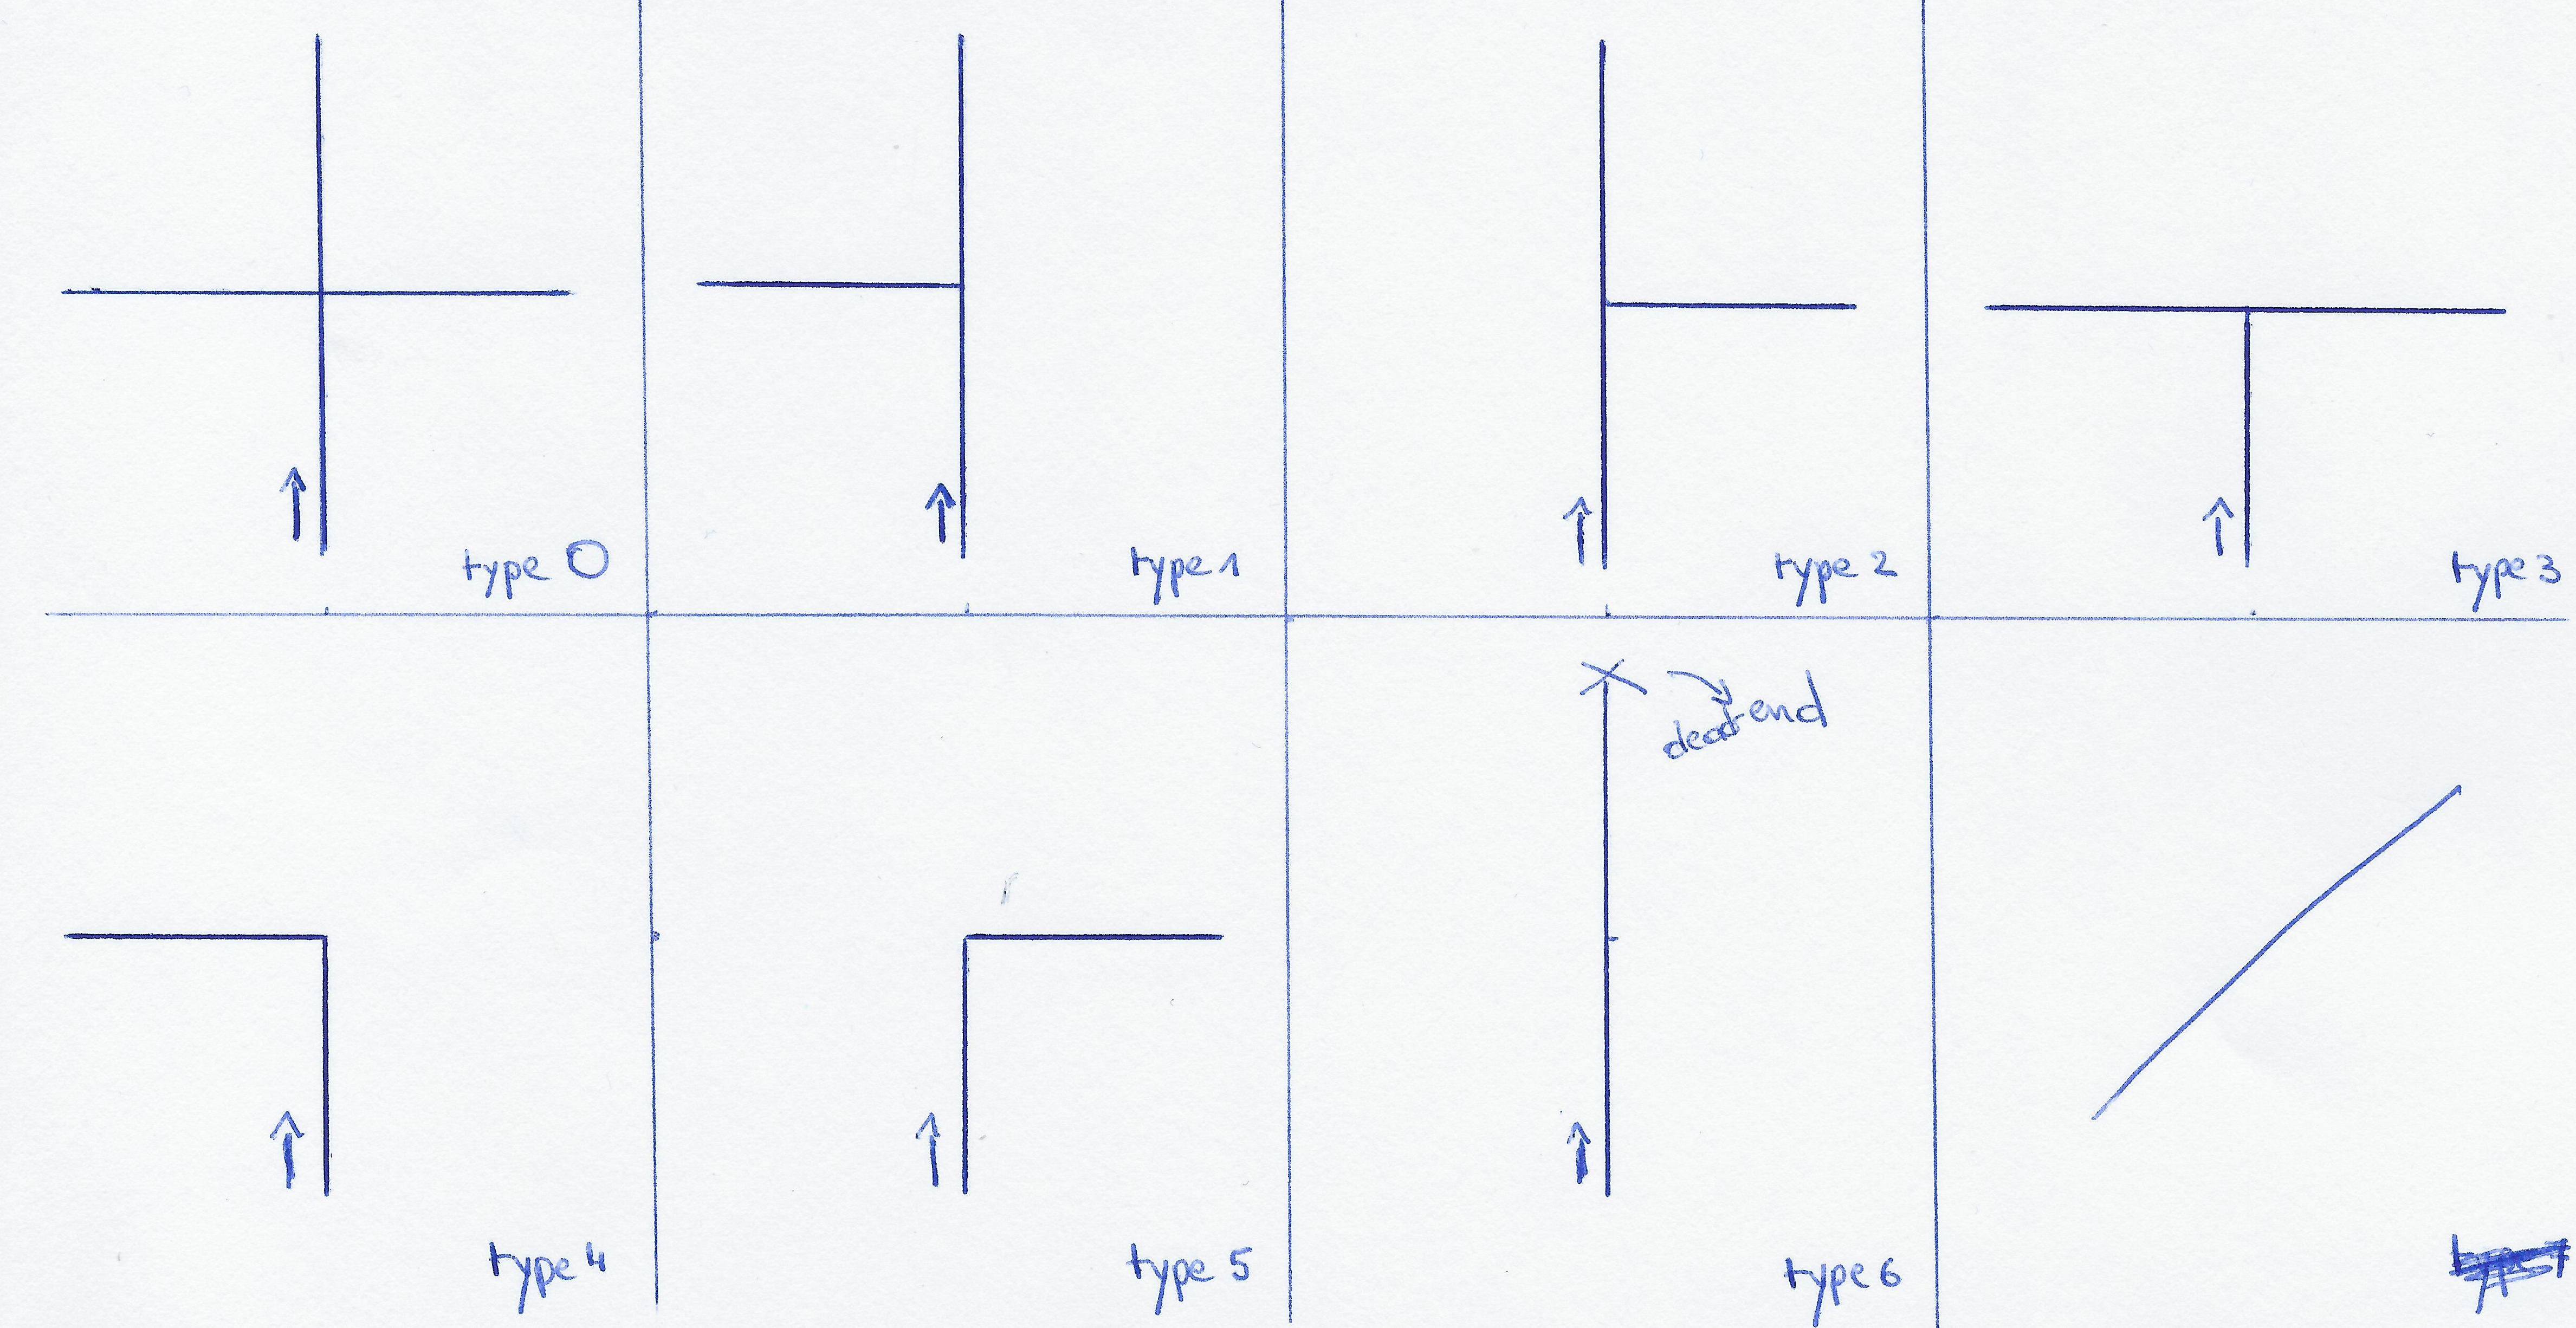
\includegraphics[scale=0.06]{figures/type-intersection}
\caption{The 7 types of intersections}
\label{fig:type-intersection}
\end{figure}
\end{frame}

%------------------------------------------------

\begin{frame}[label={frame:align}]
\frametitle{Exploration \& Mapping}
\framesubtitle{Turning \& alignment (1/2)}
(TODO: write explanation)
Explain simulated for less tedious tuning.
Compute quadratic interpolation to fi points $(\pm2,v_{init})$ and $(\pm\epsilon,v_{min})$.
$$
v(x;a,b) = a(x-\epsilon)^2+b 
$$
with initial conditions $v(x_{init}) = v_{init}$ and $v(\epsilon) = v_{min}$. Thus
$$
a = \frac{v_{init}-v_{min}}{(2-\epsilon)^2}
\qquad\text{with}\qquad
b = v_{init}
$$
\end{frame}
%\begin{multicols}{2}
%------------------------------------------------

\begin{frame}
\frametitle{Exploration \& Mapping}
\framesubtitle{Turning \& alignment (2/2)}
(TODO: write explanation)
\begin{figure}[hbtp]
\centering
\includegraphics[scale=0.07]{figures/turn-align}
\caption{Quadratic decay}
\label{fig:quad-decay}
\end{figure}
Quadratic is too short time to be applied. Better setpoint would be x instead of v.
\end{frame}

%------------------------------------------------
\section{Code} 
%------------------------------------------------

\begin{frame}
\frametitle{Overview}
\tableofcontents[currentsection,subsectionstyle=shaded]
\end{frame}

%------------------------------------------------
\begin{frame}
\frametitle{Code}
\framesubtitle{General architecture}
\begin{figure}[hbtp]
\centering
\includegraphics[scale=0.38]{figures/architecture.png}
\caption{Architecture of the code}
\label{fig:architecture}
\end{figure}
\end{frame}


%------------------------------------------------

\begin{frame}
\begin{figure}[hbtp]
\centering
\includegraphics[scale=0.1]{figures/bye-bye.jpeg}
\end{figure}
\end{frame}

%----------------------------------------------------------------------------------------

\end{document}
